\section{Tweet Author-Topic Model (with per-word topics)}

\begin{figure}[tb]
    \centering
    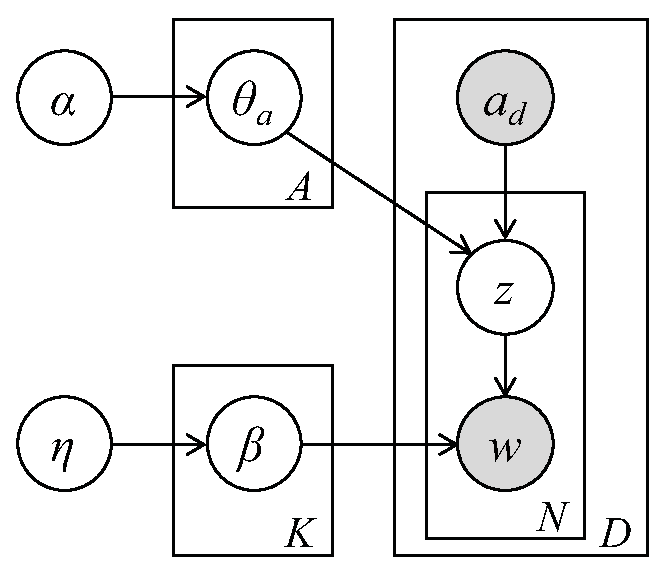
\includegraphics[width=0.4\textwidth]{TATM2.eps}
    \caption{TATM2 in plate notation}
    \label{fig:TATM2}
\end{figure}

The model is shown in Figure \ref{fig:TATM2}. The generative process is as follows:

\begin{enumerate}
	\item For $k \in {1, \ldots, K}$:
	\begin{itemize}
		\item Draw topic $\beta_k \sim \text{Dir}_V(\eta)$.
	\end{itemize}
	\item For $a \in {1, \ldots, A}$:
	\begin{itemize}
		\item Draw author's topic proportions $\theta_a \sim \text{Dir}_K(\alpha)$.
	\end{itemize}
  \item For each document (tweet) $d \in {1, \ldots, D}$:
	\begin{itemize}
		\item For each word $w \in {1, \ldots, N}$:
		\begin{itemize}
			\item Draw topic assignment $z_{d,n} \sim \text{Mult}_K(\theta_a)$.
			\item Draw word $w_{d,n} \sim \text{Mult}_V(\beta_{z_{d,n}})$.
		\end{itemize}
	\end{itemize}
\end{enumerate}


Given the hyperparameters $\alpha$ and $\eta$, the joint distribution of topics $\beta$, author-topic mixture $\theta$, topic assignments $\mathbf{z}$ and words $\mathbf{w}$ is given by:

\begin{equation}
p(\theta,\beta,\mathbf{z},\mathbf{w}|\alpha,\eta) = p(\theta|\alpha) p(\beta|\eta) \prod_{n=1}^{N}{p(z_n|\theta)p(w_n|z_n,\beta_{z_{d,n}})}
\end{equation}


\subsection{Complete conditionals}

First, we denote $\theta_a$ to be the topic proportions of the author $a$ of document $d$, i.e. $\theta_a = \theta_{a_d}$.

\textbf{Local hidden variables.} The complete conditional of the topic assignment $z_{d,n}$ is a multinomial,

\begin{equation}
p(z_{d,n} = k | \theta_a, \beta, w_{d,n}) \propto \exp \{ \log \theta_{a,k} + \log \beta_{k,w_{d,n}} \}
\end{equation}

\textbf{Global hidden variables.} In contrast with standard LDA, the topic proportions are now a global hidden variable.
The complete conditional of the author-topic proportions is a posterior Dirichlet,

\begin{equation}
p(\theta_a | \beta, z_{d}) = \text{Dir} ( \alpha + \sum_{d \in D_a}{\sum_{n=1}^{N}{z^k_{d,n}}}),
\end{equation}

\noindent where $D_a$ is the set of documents whose author is $a$.

Finally, the complete conditional for the topic $\beta_k$ is also a posterior Dirichlet,

\begin{equation}
p(\beta_k | \mathbf{z}, \mathbf{w}) = \text{Dir} ( \eta + \sum_{d=1}^{D}{\sum_{n=1}^{N}{z^k_{d,n}w_{d,n}}})
\end{equation}



\subsection{Variational parameters for batch variational inference}

The variational parameters are:
\begin{itemize}
	\item Global per-topic Dirichlets $\lambda_{1:K}$
	\item Global per-author Dirichlets $\gamma_{1:A}$
	\item Local per-word multinomials $\phi_{1:D,1:N}$
\end{itemize}

Each update of the local variables is defined as
\begin{equation}
\phi_{d,n} \propto \exp \{ \Psi(\gamma_a) + \Psi(\lambda_{.,w_{d,n}}) - \Psi(\sum_{v}{\lambda_{.,w_{d,n}}}) \}
\end{equation}

Each update of the global variational Dirichlets is defined as
\begin{equation}
\gamma_a = \alpha + \sum_{d \in D_a}{\sum_{n=1}^{N}{\phi_{d,n}}}
\end{equation}

\begin{equation}
\lambda_k = \eta + \sum_{d=1}^{D}{\sum_{n=1}^{N}{\phi^k_{d,n}w_{d,n}}}
\end{equation}



\subsection{Stochastic variational inference}


Each update of the local variables $\phi^k_{d,n}$ is then defined as
\begin{equation}
\phi^k_{d,n} \propto \exp \{ \mathbb{E}[\log \theta_{a,k}] + \mathbb{E}[\log \beta_{k,w_{d,n}}] \} + \exp \{ \mathbb{E}[\log \theta_{d,k}] + \mathbb{E}[\log \beta_{k,w_{d,n}}] \}.
\end{equation}

During the updates of local variables, we utilize an intermediate local variable $\theta_{d}$, linked to an intermediate variational parameter $\hat{\gamma}_d$. This mechanism serves as a proxy for the convergence of $\phi_{d}$ during the inner loop of the E-step. After each update of $\phi_{d}$, $\hat{\gamma}_d$ is updated as
\begin{equation}
\hat{\gamma}_d = \alpha + \sum_{n=1}^{N}{\phi_{d,n}}
\end{equation}

After fitting the local variables, we set the intermediate topics as
\begin{equation}
\hat{\lambda}_k = \eta + D \sum_{n=1}^{N}{\phi^k_{d,n}w_{d,n}}
\end{equation}

Finally, the global topics and the global per-author topic proportions are updated as
\begin{equation}
\lambda^{(t+1)}_k = (1 - \rho_t) \lambda^{(t)}_k + \rho_t \hat{\lambda}_k
\end{equation}

\begin{equation}
\gamma^{(t+1)}_a = (1 - \rho_t) \gamma^{(t)}_a + \rho_t \hat{\gamma}_d
\end{equation}




\begin{algorithm}[tb]
\caption{Stochastic variational inference for TATM2}
\label{alg:stoch_tatm2}
\begin{algorithmic}[1]
	\STATE Initialize $\lambda^{(0)}$ randomly.
	\STATE Initialize $\gamma^{(0)} = \alpha$.
	\REPEAT
	\STATE Sample a document $d$ from the data set.
	\STATE Initialize intermediate local topic proportion $\hat{\gamma}_d = \theta_{a}$.
		\REPEAT
			\FOR {$n \in \{ 1, \ldots, N \}, k \in \{ 1, \ldots, K \}$}
					\STATE Set $\phi^k_{d,n} \propto \exp \{ \mathbb{E}[\log \theta_{a,k}] + \mathbb{E}[\log \beta_{k,w_{d,n}}] \} + \exp \{ \mathbb{E}[\log \theta_{d,k}] + \mathbb{E}[\log \beta_{k,w_{d,n}}] \}$.
			\ENDFOR
			\STATE Set $\hat{\gamma}_d = \alpha + \sum_{n=1}^{N}{\phi_{d,n}}$.
		\UNTIL{$\hat{\gamma}_d$ converges}
		\STATE Set intermediate topics $\hat{\lambda} = \eta + D \sum_{n=1}^{N}{\phi_{d,n}w_{d,n}}$.
		\STATE Set global topics $\lambda^{(t+1)} = (1 - \rho_t) \lambda^{(t)} + \rho_t \hat{\lambda}$.
		\STATE Set global per-author topic proportions $\gamma^{(t+1)}_a = (1 - \rho_t) \gamma^{(t)}_a + \rho_t \hat{\gamma}_d$.
	\UNTIL{forever}
\end{algorithmic}
\end{algorithm}
